\documentclass[letterpaper,11pt]{article}

\usepackage{graphicx} % Required for inserting images

\usepackage{geometry}

\usepackage[backend=biber,style=ieee,]{biblatex}
\addbibresource{bibliography.bib}

\usepackage{setspace}
\doublespacing

\usepackage{hyperref}
\hypersetup{
    colorlinks=true, %set true if you want colored links
    linktoc=all,     %set to all if you want both sections and subsections linked
    linkcolor=black,  %choose some color if you want links to stand out
}

\renewcommand*{\thesubsection}{\alph{subsection}.}
\renewcommand*{\thesubsubsection}{\roman{subsubsection}.}

\title{My Super Duper Important Paper Thing on Air Mooscleys}
\author{Jakeypoon}
\date{March 2023}

\begin{document}

\maketitle

\newpage

\tableofcontents

\newpage

\section{Abstract}

\section{Introduction}

\section{Background}

\subsection{Braided Pneumatic Actuator}

\subsection{Length Sensor VL53L0X}

\subsection{Models}

\section{Methodology}

\subsection{Length Sensor characteristics}

The length sensor used in this research is the VL53L0X manufactured by ST (cite) in an LGA package. The sensor uses a VCSEL emitter to generate 940nm wavelength light pulses. The reflected light is measured with a collector to determine the distance of a target by using the time of flight. The sensor has a range of 2 meters and a resolution of 1 millimeter. The main communication protocol used for this sensor is I2C. ST provides an C API for the user, but it will not be used directly in this research. The C API is instead repackaged into an Arduino library to be used with the Teensy 4.1 controller board, which is the primary electronic interface with all sensors, pressure control, and data collection.\\

Pololu designs and manufactures the sensor carrier for the VL53L0X.  The carrier board also incorporates a voltage regulator to shift the voltage requirement of the VL53L0X from 2.8V to 3.3V or 5V which is easier to interface with the Teensy 4.1. The dimension of the carrier board is 12.7mm X 17.8mm X 2.16m6m. The board has 6 signals available: VDD, VIN, GND, SDA, SCL, XSHUT, and GPIO1.

\begin{figure}[h]
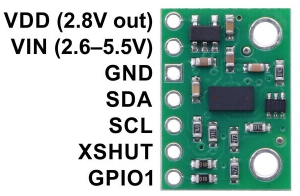
\includegraphics[width=5cm]{chip}
\centering
\end{figure}

For the purpose of this research, the VDD and GPIO1 pins are not used; the SDA and SCL pins are used for I2C communication with the controller; XSHUT is used to change sensor ID when multiple sensors are mounted on the same bus. Multiple sensors can be used with the same controller with the sacrifice of sampling frequency. The compact footprint of the board is ideal for implementing with the 20mm diameter Festo fluidic muscle. To adapt the VL53L0X for smaller diameter muscles, a custom design of the VL53L0X LGA circuit would have to be created. Only the 20mm-diameter muscle was used in this research to show the feasibility and performance of such sensing mechanism in measuring BPA length.\\

The sensor is advertised to be independent to the target surface’s reflectivity. However, during testing of the sensor, it was found that the surface’s reflectivity boosts sensor accuracy inside the muscle.

\subsubsection{Sensor drift and variation}

The sensor is tested outside of the muscle to determine sensor drift and variation. The target is a PLA 3D printed surface 15mm away from the sensor. For this drift test, the sensor is sampled at 20Hz for 3 minutes. The data is written to the serial port and read by a MATLAB program [cite MATLAB program]. To determine drift rate of the sensor, the MATLAB linear fit algorithm polyfit is used and the drift rate is the slope of the linear fit. The variation of the sensor is the standard deviation within the data collection window.

\subsubsection{Noise filtering}

To reduce the sensor noise, a discrete second-order low-pass Butterworth filter is used in real-time to filter the incoming data. The frequency response of BPA was found to be about two Hertz [X Kingsley, Quinn 2002], which is close to the cut-off frequency found in human ranging from 1.7-3.1 Hz [Brerton \& McGill, 1998]. The cut-off frequency of the Butterworth filter needs to be sufficient to filter out external noise, but not interfering with the response frequency of the BPA. The cut-off frequency of the Butterworth filter is set to 5 Hz with no additional gain and tested on BPA set up in atmosphere. The filter is derived from the standard form of the continuous Butterworth filter. The transfer function of the filter in the continuous domain is

\begin{equation}
    G_c(s)=\frac{\omega^2_c}{s^2+2 \zeta w_cs+w^2_c}
\end{equation}

where $\omega_c$ is the corner frequency is rad/s and $\zeta$ is the damping factor. The damping factor for a second order Butterworth filter is 0.707 [cite], and the corner frequency is 5 Hz. Substituting the values in equation 1, we get the transfer function in the continuous domain.

\begin{equation}
    G_c(s)=\frac{631.7}{s^2+35.54s+631.7}
\end{equation}

\subsection{Leak Test}

Blah blah blah \cite{jordan} blah blah blah blah.

\subsection{Calibration}

\subsection{Dynamic Testing}

\section{Results}

\subsection{Performance in atmospheric}

\subsection{Performance inside muscle with filtering and calibration}

\subsection{Dynamic Performance}

\subsection{Reflectivity}

\section{Discussion and Conclusion}

\subsection{Reflectivity}

\subsection{Length sensing in general}

\section{Future Work}

\printbibliography

\end{document}
